\documentclass{article}
\usepackage[utf8]{inputenc}
\usepackage[italian]{babel}

\usepackage[a4paper, total={6.5in, 10in}]{geometry}
\usepackage{setspace}

\usepackage{listings}
\usepackage{xcolor}
\usepackage{hyperref}

\usepackage{graphicx}


\newcommand{\floor}[1]{\lfloor #1 \rfloor}

\lstset{
  language=C++,
  backgroundcolor=\color{black!5}, % set backgroundcolor
  columns=fullflexible,
}

\title{Competitive Programming}
\author{Riccardo Maso Davide Guidobene Florian Sabani Davide Cazzin}
\date{Novembre 2021}

\onehalfspacing
\begin{document}

\maketitle

\section{Problemi}

Con la Competitive Programming definiamo l'attività' per la quale andiamo a risolvere un problema strutturato in modo tale da avere : 

\begin{enumerate}
    \item Descrizione Testuale del problema
    \item Definizione del File Input
    \item Input Constraint
    \item Esempio di Input/Expected Output 
    \item Time \& Space Constraint (TL \& SL)
\end{enumerate}

Lo scopo del programmatore competitivo e' quello di leggere il testo del problema, analizzarne la complessità e svilupparne una soluzione in grado di dato l'input, fornire sempre l'output atteso, rientrando nei limiti delle risorse tempo e spazio che l'algoritmo può usare.

Es :\url{https://open.kattis.com/problems/hello} \url{https://open.kattis.com/problems/10kindsofpeople}

\section{Classi di complessità}
[parlare della BigO Notation]\newline
Per poter risolvere i problemi rientrando nel TL dobbiamo fare leva sull' Input Constraint datoci dalla descrizione del problema.In particolare avendo N la dimensione dei dati in input, generalmente possiamo scegliere un algoritmo risolutivo seguendo quanto dice la seguente tabella : 

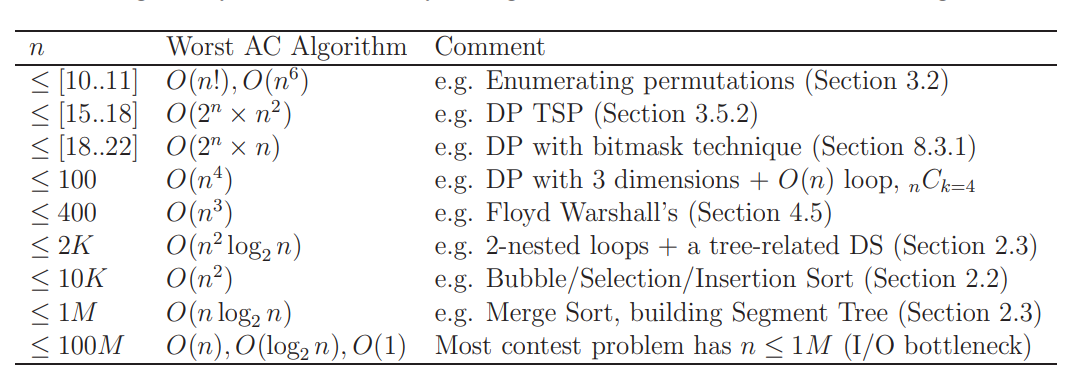
\includegraphics[scale=0.5]{matrix.PNG}

\section{Quale linguaggio?}

\# C/C++ Python Java

\section{Read/Write}

Sempre attenzione nel rendere operazioni I/O efficienti.

\begin{lstlisting}
// Read something
int value;
cin >> value;

// Print something
cout << value << "\n";
cout << value << endl; // with flush 

\end{lstlisting}


\section{Template}

\lstinputlisting{template.cpp}

\section{Vector}


\section{Sort}

In competitive programming molto difficilmente dovremmo scrivere un algoritmo di sorting, la maggioranza delle volte useremo il sort che ci viene fornito dalla standard library.

\begin{lstlisting}
void sort (RandomAccessIterator first, RandomAccessIterator last);

void sort (RandomAccessIterator first, RandomAccessIterator last, Compare comp);
\end{lstlisting}

Il sort utilizzato da questa funzione è chiamato IntroSort e ha una complessità temporale $O(nlog(n))$ e spaziale $O(log(n))$.

Il comparator di default che viene utilizzato dalla funzione sort, nel caso non ne venga fornito un altro, è $less<int>$ e ordina gli elementi presenti all'interno della struttura dati in ordine non decrescente. Per ordinare il vettore con ordine non crescente possiamo usare il comparator $greater<int>$, come nel seguente esempio:

\begin{lstlisting}
    vector<int> v = {1,4,5,6,3,2};
    sort(v.begin(), v.end(), greater<int>);
\end{lstlisting}

Nel caso volessimo ordinare il nostro vettore secondo un criterio diverso da quello del comparator $less<int>$ e $greater<int>$ allora dobbiamo definire un comparator. Supponiamo ad esempio di aver un vettore di $pair<string, int>$ e vogliamo che il vettore sia ordinato in base all'intero con ordine non decrescente e nel caso di interi uguali devono essere ordinati in ordine alfabetico.

\section{Struct}

\end{document}
